
%% !TEX root = manual.tex

\begin{figure}[h!]
\centering
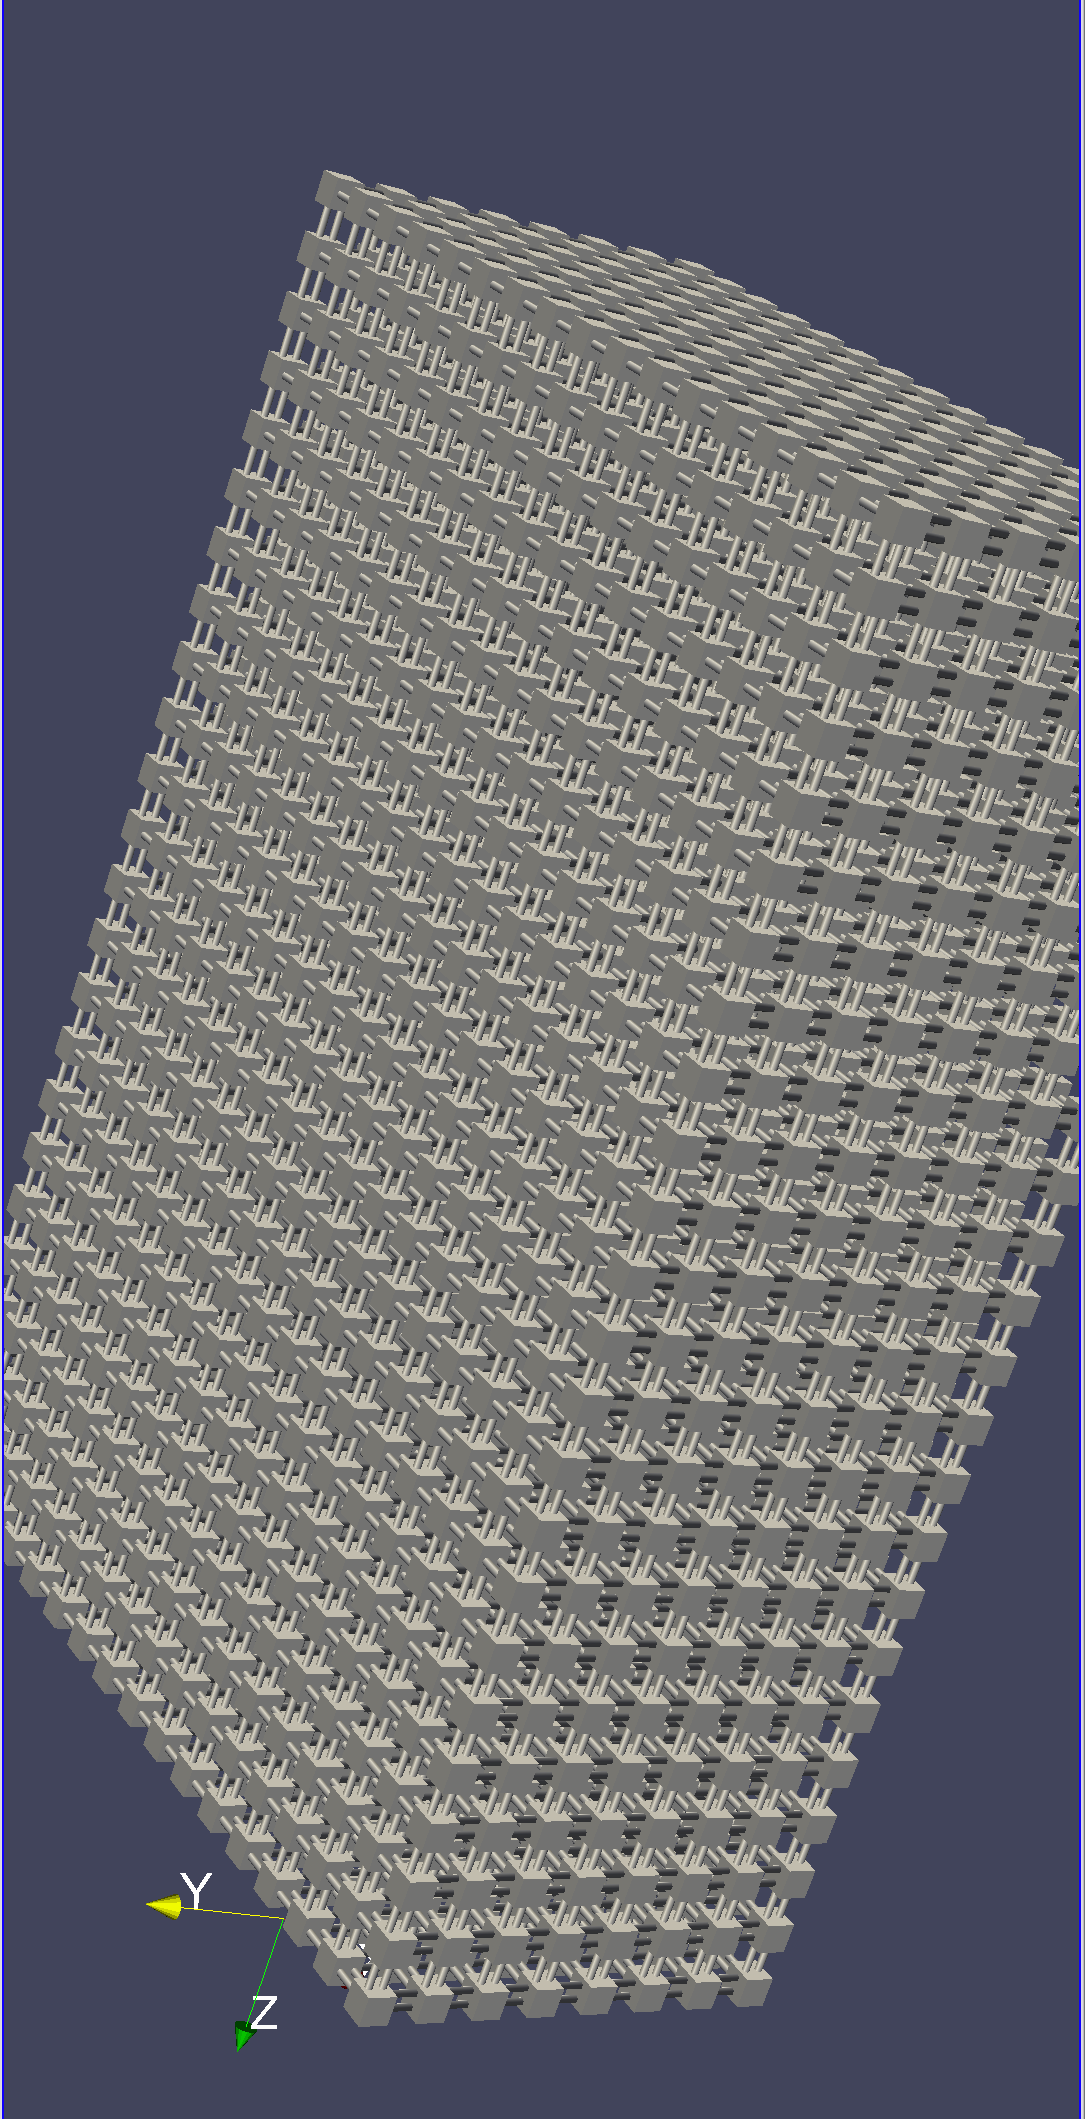
\includegraphics[angle=90, width=0.9\textwidth]{figures/vtk/hopper.png}
\caption{3D model of Hopper in Paraview}
\label{fig:vtk}
\end{figure}


\section{Visualization with VTK}
\label{sec:tutorials:vtk}

\sstmacro has built-in support for doing 3D modeling with VTK $>=$ 6.0 from Kitware.  First, download and install VTK 6.0, currently at \url{http://www.vtk.org/VTK/resources/software.html}.   You must configure \sstmacro with the version number and the install location you chose when building VTK.

\begin{ShellCmd}
sstmacro/build$ ../configure --prefix=/usr/sstmacro --with-vtk=6.0 --with-vtk-path=path_to_vtk 
\end{ShellCmd}
If \inlineshell{--with-vtk-path} is omitted, it defaults to \inlineshell{/usr/local}.  Due to subtleties in the VTK installation, you MUST specify the version number.

To generate the visualization, you'll want to add the following parameters to the parameter file you use:

\begin{ViFile}
vis_engine = vtk
vis_update = 1000ns
\end{ViFile}

The \textit{vis\_engine} parameter tell \sstmacro to open a VTK window.  The \textit{vis\_update} parameter tells \sstmacro how often, in simulation time, to update the visualization.  Note that this could make your simulation run much slower if your vis\_update is small (many updates), or make the visualization choppy if vis\_update is too large.  
Finally, you need to modify your library load path (DYLD\_LIBRARY\_PATH for Mac, LD\_LIBRARY\_PATH for Linux) to include the location of the installed VTK libraries, like so:

\begin{ShellCmd}
... $ export DYLD_LIBRARY_PATH=/usr/lib/
\end{ShellCmd}

Running a simulation with a VTK-enabled parameter file will open a window that shows the 3D model in real time.  \sstmacro execution will become interactive, requiring a keystroke on the terminal for both starting and stopping the simulation (so you can be ready to view it).   However, the visualization itself is not yet interactive (you can't change the viewing angle). However, \sstmacro will also produce a file called interconnect-start.vtp, which can be opened with Paraview (also from Kitware), which allows you to move the camera around and step through time.  Figure \ref{fig:vtk} shows a screenshot of the visualization of Hopper brought up in Paraview.  In addition, you can set the \textit{vis\_file\_update} parameter to a simulation time interval, which outputs a model file at each interval that can be replayed in Paraview. 



\subsection{Currently supported features}

\sstmacro currently only supports VTK visualization when using the following network topologies:

\begin{itemize}
\item 3D torus
\item Dragonfly - global links only
\end{itemize}

\sstmacro also only supports VTK visualization when using the the following network models:

\begin{itemize}
\item cycle\_accurate - links show individual output buffer occupancy.  Switches show total input buffer occupation. 
\item packet - links show measured link bandwidth. Switches show total switch input bandwidth.
%\item fastflower -
\end{itemize}